\documentclass[11pt]{article}
\usepackage[a4paper,margin=1in]{geometry}
\usepackage{amsmath,amssymb}
\usepackage{booktabs}
\usepackage{graphicx}
\usepackage{xcolor}
\usepackage{hyperref}
\hypersetup{colorlinks=true,linkcolor=blue,urlcolor=blue}
\newcommand{\rt}[1]{\texttt{#1}}
\newcommand{\fn}[1]{\texttt{#1}}
\newcommand{\oeis}[1]{\href{https://oeis.org/#1}{\texttt{#1}}}
\providecommand{\ket}[1]{|#1\rangle}
\providecommand{\bra}[1]{\langle #1|}

\title{\textbf{Report R5 --- Dissipative rules: recurrent classes, attractors,
protected coherence, and growth laws}\\
\large Krylov sector analysis of quantum cellular automata (Tier 1a/1b/1c)}
\author{QCA Sector Analysis project (Tier 1)}
\date{2026-07-22 \quad\small(engine\_version \texttt{1a.1})}

\begin{document}
\maketitle

\begin{abstract}
We extend the exact pipeline to the 240 dissipative quantum cellular automata
(rules containing a reset channel $\rt D$ or $\rt E$). The one-cycle channel is
now genuinely non-unitary: the directed transition graph has \emph{transient}
strongly connected components flowing into \emph{recurrent classes}. We sweep
all dissipative rules (both boundary conventions, $N=6\ldots13$), census their
attractor structure, classify each recurrent class by the peripheral spectrum of
its exact restricted superoperator (Tier 1b), and --- new in this revision ---
extract the \emph{growth laws} of the attractor count and the largest attractor
(Tier 1c). Two results organise the report. First, the transition graph is not a
lossy picture of the channel but the \emph{exact} description of a different
experiment (the monitored QCA), and it fails to describe the unmonitored channel
in a way we can now census exactly: for $92$ of $240$ \rt{pbc} rules the
channel's attractor is not spanned by computational-basis states at all, and
every one of those rules contains a Hadamard, while all $80$ Hadamard-free
dissipative rules are basis-spanned without exception. Second, dissipative
growth is far from generic: $94$ of the \rt{pbc} series ($123$ \rt{obc0}) satisfy
an \emph{exact} integer linear recurrence, so their growth bases are algebraic
numbers --- $\varphi$, $\sqrt3$, the supergolden and plastic constants --- rather
than fitted slopes.
\end{abstract}

\section{Dissipative graph structure}
For a dissipative rule the channel $\Phi_C(\rho)=\sum_\mu K_\mu\rho K_\mu^\dagger$
has $\ge 2$ Kraus operators. The exact engine propagates every Kraus branch
(never merging incoherent alternatives) and records the directed transition
graph $M_{yx}=\sum_\mu|\langle y|K_\mu|x\rangle|^2$. Its terminal strongly
connected components are the recurrent classes; non-terminal components are
transient. We record, per $(\text{rule},N,\text{bc})$: the number and sizes of
recurrent classes, the transient depth (longest condensation-DAG path), and the
basin structure. The engine and its dissipative branch machinery are validated
against an independent dense-channel oracle (528/528 support checks; per-site
Kraus completeness $A_0^\dagger A_0+A_1^\dagger A_1=\mathbb{1}$).

\subsection{What actually fires each cycle: neighbour-controlled Kraus operators}
\label{sec:kraus}
Saying that ``the reset channels fire every cycle'' is true only in the weak
sense that every site is \emph{addressed} every cycle; whether anything happens
to it is decided by its two neighbours. Within one brickwork sublayer the sites
being acted on are mutually non-adjacent, so the neighbours of an active site lie
in the \emph{other} sublayer and are untouched while it acts. The sublayer is
therefore a genuinely \emph{controlled} channel: writing
$P^{(mn)}_i=\ket m\!\bra m_{i-1}\otimes\ket n\!\bra n_{i+1}$ for the projector on
the neighbour pair, the site-$i$ Kraus operators are
\begin{equation}
  K^{(i)}_\mu \;=\; \sum_{m,n\in\{0,1\}} P^{(mn)}_i\, c^{(mn)}_\mu\, P^{(mn)}_i ,
  \label{eq:pdp}
\end{equation}
with the local symbol $r_{mn}\in\{\rt I,\rt V,\rt D,\rt E\}$ fixing the branches
\begin{center}\small
\begin{tabular}{ll}
$\rt I$: & $c_0=\mathbb 1$ \\
$\rt V$: & $c_0=H$ \\
$\rt D$: & $c_0=\ket0\!\bra0,\quad c_1=\ket0\!\bra1$ \\
$\rt E$: & $c_0=\ket1\!\bra1,\quad c_1=\ket1\!\bra0$
\end{tabular}
\end{center}
(the two branches of a reset record whether the centre had to be de-excited).
Each summand of \eqref{eq:pdp} literally reads \emph{projector--decay--projector}:
the neighbour projector selects the configuration, the local map acts, and the
projector still holds afterwards because $P^{(mn)}_i$ commutes with everything
supported on site $i$ alone. That commutation is what makes the control
\emph{classical within a sublayer} --- the conditioning register is never
disturbed by the operation it conditions --- and it is the reason the Kraus
branch label $\mu$ can be carried around as a per-site classical record at all.
The practical consequence is that dissipation here is not a rate: a rule with
$r_{00}=\rt D$ and $\rt I$ elsewhere acts as the identity on any configuration
containing no $000$ pattern, so which rules are strongly damped is a statement
about the \emph{local patterns} the state contains, not about a coupling
constant.

\paragraph{What $M$ is, exactly.} It is worth being precise about the status of
$M$, because the usual phrase ``the graph is an approximation'' is wrong in a
way that matters. $M$ is the transition matrix of the QCA \emph{monitored in the
computational basis after every cycle}: measure all $N$ qubits at the end of each
brickwork cycle and $M$ gives the exact conditional distribution of outcomes. So
$M$ is not an approximation of anything --- it is the exact dynamics of a
different (and physically realisable) experiment. What it cannot do is predict
the \emph{unmonitored} channel, because there coherences feed back into
populations between cycles. Everything below is a statement about how far apart
those two experiments are, rule by rule.

\paragraph{Individual trajectories versus the graph.} The distinction is easiest
to state at the level of single trajectories, and it is not the usual
``trajectories average to the channel'' remark. A trajectory of the
\emph{unmonitored} channel is a sequence of Kraus labels $\mu$, one per site per
cycle. Between resets the conditional state is \emph{not} a basis state: $\rt V$
is a Hadamard, so a trajectory generically carries superpositions, and the
operators applied later in the same cycle are controlled by neighbours that are
themselves in superposition. Equation~\eqref{eq:pdp} then acts as a
\emph{coherently controlled} gate --- a partial swap of amplitude between the
neighbour-configuration branches --- rather than as a classical if-then. The
branch probability of the next label depends on the accumulated amplitudes, i.e.\
on the whole measurement history, so an unmonitored trajectory is a walk on a
continuum of rays, not on $2^N$ labels. (This is exactly why the ``ray graph''
repair fails: rules 22 and 50 already exceed $6\times10^4$ distinct rays at
$N=3$, where the basis graph has $8$ nodes.)

In the \emph{monitored} experiment all $N$ qubits are measured at the end of each
cycle. The state is projected onto a basis label, so the next cycle's branch
probabilities depend on that label alone and nothing else --- which is precisely
the Markov property, with kernel $M_{yx}$. Two things are destroyed: coherence
generated by $\rt V$ never survives into the following cycle, and the trajectory
ensemble is re-collapsed to populations once per cycle. Note that $M$ is
\emph{not} the ``dephase after every gate'' chain: within a cycle the Hadamards
and the controlled resets act coherently, and only the end-of-cycle measurement
intervenes. Consequently $M$ reproduces the unmonitored channel's populations
exactly iff no coherence created in one cycle can influence populations in the
next, which happens precisely when every Kraus operator is a $0/1$ partial
permutation --- i.e.\ when the rule is Hadamard-free. That criterion is confirmed
without exception in \S\ref{sec:failures}: all $80$ $\rt V$-free dissipative
rules are basis-spanned, and every rule that is not contains a $\rt V$.

\section{Census of attractor structure}
\label{sec:census}
Table~\ref{tab:census} classifies every dissipative rule by the structure of $M$
at the largest computed $N$: a unique classical fixed point, several point
attractors (multistability, signalling a basis-diagonal conserved charge), or one
or more extended ($>\!1$-state) attractors.
\begin{table}[h]\centering\small\begin{tabular}{@{}l rr@{}}
\toprule
attractor structure & obc0 & pbc \\
\midrule
unique fixed point & 26 & 16 \\
multistable (point attractors) & 23 & 13 \\
single extended attractor & 24 & 31 \\
multiple extended attractors & 8 & 21 \\
\midrule
total dissipative rules & 81 & 81 \\
\bottomrule
\end{tabular}

\caption{Dissipative rules by attractor structure of the monitored chain $M$ and
boundary convention.}
\label{tab:census}\end{table}

Two ground-truth items (context \S8) are reproduced: rule 22 $(\rt{IVVD})$ on
\rt{pbc} at even $N$ has exactly three point attractors (the vacuum and the two
N\'eel states); rules 28/29 illustrate the boundary/wall-transparency contrast.

\section{Tier 1b: attractor types}
For each recurrent class $R$ we build the \emph{exact} restricted superoperator
$\Phi_R$ on $\mathrm{span}(R)\otimes\mathrm{span}(R)^*$ from the labelled Kraus
branches, and read its peripheral spectrum (geometric multiplicities, robust to
the non-normal transient Jordan structure). A class is \emph{mixing} (a unique
steady state; a classical pointer/dark state when $|R|=1$), a \emph{limit cycle}
(peripheral roots of unity, basis-diagonal eigenoperators), or
\emph{coherence-carrying} (a decoherence-free subsystem of dimension $d_k>1$).
\begin{table}[h]\centering\small\begin{tabular}{@{}rl r l l@{}}
\toprule
W & tuple & \#recur & attractor kinds & max $d_k$ \\
\midrule
0 & \texttt{DDDD} & 1 & 1$\times$mixing & 1 \\
1 & \texttt{VDDD} & 1 & 1$\times$unresolved & 1 \\
22 & \texttt{IVVD} & 3 & 3$\times$mixing & 1 \\
28 & \texttt{IIVD} & 11 & 3$\times$mixing, 8$\times$coherent & 3 \\
29 & \texttt{EIVD} & 10 & 2$\times$mixing, 8$\times$coherent & 3 \\
50 & \texttt{DVVV} & 1 & 1$\times$mixing & 1 \\
76 & \texttt{IIID} & 131 & 131$\times$mixing & 1 \\
178 & \texttt{DVVE} & 2 & 2$\times$mixing & 1 \\
200 & \texttt{DIII} & 90 & 90$\times$mixing & 1 \\
232 & \texttt{DIIE} & 46 & 46$\times$mixing & 1 \\
\bottomrule
\end{tabular}

\caption{Tier-1b attractor classification (pbc, $N=8$). Rule 28 carries
coherence-protecting extended attractors ($d_k>1$); most others relax to
classical pointer states.}
\label{tab:tier1b}\end{table}

\section{Strong vs.\ weak symmetry: what each stage can see}
\label{sec:strongweak}
A \emph{strong} symmetry commutes with every Kraus operator individually; a
\emph{weak} symmetry only makes the channel covariant (context \S5). For unitary
rules there is a single Kraus operator and the two coincide. This pipeline does
\textbf{not} detect symmetry \emph{operators} (no commutant of $\{K_\mu\}$, no
charge null-space --- that is Tier 2); it separates the two \emph{operationally}:

\begin{itemize}
  \item \textbf{Tier 1a (graph).} $M$ is the monitored chain. Only
  basis-diagonal \emph{strong} charges fragment it; their signature is the number
  of recurrent classes (Table~\ref{tab:census}). This is the only symmetry
  information the graph carries.
  \item \textbf{Tier 1b (channel).} The exact Cesaro rank
  $\dim\mathrm{Fix}(\Phi)$ (geometric multiplicity of eigenvalue 1 of the full
  $4^N$ superoperator) sees the coherent fixed-point algebra. Weak symmetries and
  protected coherences appear here and \emph{only} here.
\end{itemize}
The gap $\dim\mathrm{Fix}(\Phi)-\sum_R\dim\mathrm{Fix}(\Phi_R)\ge 0$ measures what
the monitored description misses (Table~\ref{tab:cesaro}).

\section{When the graph cannot name the attractor: two distinct failure modes}
\label{sec:failures}
\label{sec:failure}
The earlier revision of this report reported a single number --- ``38 of 240
rules are unfaithful'' --- from a leakage test. That test is the weaker of two,
and it misses the more common failure. We now separate them.

\paragraph{Mode 1: leakage (the weak test).} Ask whether
$\Phi^{t}(\mathbb{1}/d)$ retains population on states the graph calls transient,
and whether $\mathrm{Fix}(\Phi)$ has weight outside the recurrent block. This
catches rules where the graph puts the attractor on the \emph{wrong states}:
$\mathbf{38}$ of $240$ at $N=4$, \rt{pbc} (Table~\ref{tab:faithful}). Rule 22 is
the sharp case --- fixed-point operators carry weight $0.49$ outside the
recurrent block and $\Phi^{400}(\mathbb{1}/d)$ retains $12.5\%$ of its population
on graph-``transient'' states (limit support: 11 basis states, not 3). Since
$\dim\mathrm{Fix}=25=5^2$ the true attractor is a $5$-dimensional
decoherence-free subspace, and the ``three point attractors'' are an artifact of
dephasing. Rule 50 ($\dim\mathrm{Fix}=13$, $25\%$ leaked) and rule 106 ($42\%$)
are stronger cases.

\paragraph{Mode 2: coherence (the structural test).} A rule can pass the leakage
test and still be undescribable by any state-space graph, because the graph's
vertices \emph{are} basis states: whatever it calls the attractor is a
\emph{set}, while the channel's attractor is a \emph{subspace}. The right
question is therefore whether that subspace is basis-spanned,
\[
  \dim_{\mathrm{att}} \;=\; \dim\operatorname{supp}
  \lim_{T\to\infty}\tfrac1T\sum_{n<T}\Phi^n(\mathbb{1}/d),
  \qquad
  \mathrm{coh\ dirs} \;=\; \dim_{\mathrm{att}} - \#\{\text{basis states inside}\},
\]
and $\mathrm{coh\ dirs}>0$ is exactly the structure no graph can represent.
Rule 27 $(\rt{VEVD})$ shows the two tests are genuinely different: the graph
reports $9$ recurrent states, the truth is \emph{one} pure stationary
superposition --- and the leak is $0$, so Mode 1 sees nothing. Unlike the leaked
weight, $\mathrm{coh\ dirs}$ is initial-state independent and not normalised by
$2^N$ (leakage from $\mathbb{1}/d$ gives rules 104/233 a spurious $2/2^N$ that
vanishes with $N$ for purely dilutional reasons).

The Cesaro limit must be taken to a genuine \emph{spectral gap}, not to a fixed
burn-in. With burn-in $600$, rule 19 at $N=6$ reports $\dim_{\mathrm{att}}=35$
with smallest kept eigenvalue $1.9\cdot10^{-9}$ against largest dropped
$4.8\cdot10^{-10}$: no gap, so the ``attractor'' is mostly still-decaying
transient. Converged (burn-in $4000$) it is $5$, with a gap of $1.8\cdot10^{-2}$
against $10^{-15}$. We therefore double the burn-in until
$\lambda_{\text{kept}}/\lambda_{\text{dropped}}>10^{4}$.

\paragraph{Census.} All $240$ dissipative rules, \rt{pbc}, $N=4,6,8$, every rule
converged:
\begin{center}\small
\begin{tabular}{@{}lrrr@{}}
\toprule
 & $N=4$ & $N=6$ & $N=8$ \\
\midrule
rules with a non-basis-spanned attractor & 84 & 60 & 72 \\
not converged & 0 & 0 & 0 \\
\bottomrule
\end{tabular}
\end{center}
The count is \textbf{non-monotonic} in $N$ and stays extensive: $54$ rules are
coherent at all three sizes and $92$ at some size, so this is not a small-$N$
accident that washes out. Two structural facts stand out:
\begin{itemize}
  \item \textbf{The Hadamard is necessary --- and one half of this is trivial.}
  All $80$ Hadamard-free dissipative rules ($\rt V\notin$ tuple) are basis-spanned
  at every censused size, and all $92$ coherent rules contain at least one $\rt V$.
  The first clause is not a discovery: a $\rt V$-free rule is \emph{deterministic
  on basis states} (both Kraus branches of a reset land on the same state), so it
  is an ordinary classical elementary cellular automaton and its graph is exact
  by construction --- this is exactly why we treat those $80$ rules as a
  \emph{classical baseline} (\S\ref{sec:classical}). The content is the converse:
  coherence \emph{requires} a $\rt V$, without exception.
  \item \textbf{The wall-Hadamard core.} The $12$ rules with $r_{01}=r_{10}=\rt V$
  --- $\{18,19,22,23,50,55,146,151,178,179,182,183\}$, i.e.\ Hadamard exactly on
  the domain-wall configurations --- are coherent \emph{without exception}. A
  Hadamard driven by the wall pattern rather than by the site occupation is the
  mechanism that keeps a superposition stationary.
\end{itemize}
Mode 2 also cuts across the graph-level classification of \S\ref{sec:census}:
$37$ of the $47$ \rt{pbc} rules with a single extended attractor are coherent,
against $13$ of $75$ multistable rules --- extended graph attractors are the ones
most likely not to be attractors at all in the coherent sense.

\begin{table}[h]\centering\small\begin{tabular}{@{}rl rrr l@{}}
\toprule
W & tuple & \#rec.\ states & $\dim\mathrm{Fix}(\Phi)$ & leaked weight & graph faithful? \\
\midrule
0 & \texttt{DDDD} & 1 & 1 & 0.000 & yes \\
200 & \texttt{DIII} & 10 & 100 & 0.000 & yes \\
232 & \texttt{DIIE} & 6 & 36 & 0.000 & yes \\
28 & \texttt{IIVD} & 3 & 9 & 0.000 & yes \\
76 & \texttt{IIID} & 11 & 121 & 0.000 & yes \\
22 & \texttt{IVVD} & 3 & 25 & 0.125 & \textbf{no} \\
50 & \texttt{DVVV} & 1 & 13 & 0.250 & \textbf{no} \\
178 & \texttt{DVVE} & 2 & 9 & 0.063 & \textbf{no} \\
106 & \texttt{DEIV} & 1 & 8 & 0.422 & \textbf{no} \\
\midrule
\multicolumn{6}{@{}l}{census at $N=4$, pbc: 202 faithful / 38 unfaithful of 240 dissipative rules} \\
\bottomrule
\end{tabular}

\caption{Mode-1 (leakage) test (pbc, $N=4$): leaked weight is the population of
$\Phi^{400}(\mathbb{1}/d)$ remaining on graph-transient states. Non-zero leak
means the graph misplaces the coherent attractor.}
\label{tab:faithful}\end{table}

\begin{table}[h]\centering\small\begin{tabular}{@{}rl rrr@{}}
\toprule
W & tuple & classical dim & Cesaro rank & coherence gap \\
\midrule
0 & \texttt{DDDD} & 1 & 1 & 0 \\
1 & \texttt{VDDD} & 15 & 15 & 0 \\
22 & \texttt{IVVD} & 3 & 25 & 22 \\
28 & \texttt{IIVD} & 3 & 9 & 6 \\
50 & \texttt{DVVV} & 1 & 13 & 12 \\
178 & \texttt{DVVE} & 2 & 9 & 7 \\
200 & \texttt{DIII} & 10 & 100 & 90 \\
232 & \texttt{DIIE} & 6 & 36 & 30 \\
\bottomrule
\end{tabular}

\caption{Exact Cesaro rank vs.\ the graph-resolved per-class fixed dimension
(pbc, $N=4$). A zero gap (rule 0, pure decay) is fully classical; a large gap
flags protected coherence.}
\label{tab:cesaro}\end{table}

\section{Tier 1c: dissipative growth laws}
\label{sec:scaling}
We now fit the $N$-dependence of the attractor count $\#\mathrm{att}$, the
largest attractor $D_{\max}$, the largest basin, and the transient depth for all
$240$ rules and both boundary conventions over $N=6\ldots13$ (coverage is
complete; no rule is ergodic). Two methodological points were forced by the data
and are worth recording, since they are the difference between a result and an
artifact.

\paragraph{Commensurability, and not overfitting it.} Dissipative series oscillate
with $N$ --- a \rt{pbc} chain of odd length cannot host the two N\'eel states, and
some attractors are period-$3$ density waves that only fit a ring of the right
length --- so a joint fit averages two or three different laws into a meaningless
one. We therefore split the series by $N\bmod p$ for $p\in\{2,3,4\}$, but choosing
the period is where overfitting lives: a larger $p$ has more parameters and always
fits at least as well, so any residual-based rule drifts to $p=4$. We fix $p$ by
BIC with a decisive Kass--Raftery margin ($\ge10$) and at least four points per
class, \emph{or} by an exact integer recurrence holding on every residue class ---
and only when the joint fit is actually failing. The criterion is calibrated
against a null of smooth-exponential-plus-$25\%$-noise surrogates
(\fn{scaling/overfit\_audit.py}): the naive ``smallest period that halves the
residual'' splits $21\%$ of pure noise and plain argmin-BIC splits $33\%$, while
this rule splits $3\%$, and the exact-recurrence route fired $0/4000$. On the deep
dataset ($N=6\ldots17$) this yields $33$ \rt{pbc} parity ($p{=}2$) splits and $14$
period-$3$ splits ($14$ and $14$ for \rt{obc0}); of the period-$3$ splits $12$
\rt{pbc} ($10$ \rt{obc0}) are certified by an \emph{exact} recurrence on every
residue class, not merely by BIC, so they are not fitting artifacts. No
period-$4$ claim survives at $N\le17$ (it needs $N\ge21$ to be honest). The period fixes the growth
\emph{class}, not the base --- a period-$p$ oscillation is itself an order-$p$
recurrence, so the exact-base search below already caught these on the whole
series.

\paragraph{Rate model.} The unitary pipeline fits
$\ln y = c + \alpha\ln N + \kappa N$, carrying the $\alpha\ln N$ term so that
binomial prefactors do not bias $\kappa$. On the ragged dissipative series that
model is unstable: for rule 90, $D_{\max}=1,15,1,7,3,63,2,127$ yields
$\alpha=-7.5$ and a growth base of $11.25$ --- impossible, since $D_{\max}\le2^N$
forces base $\le2$. We therefore take the growth \emph{class} from BIC model
selection but the growth \emph{rate} from the two-parameter fit
$\ln y=c+\kappa N$, which cannot trade the rate against a power, and mark a
series \emph{irregular} (no rate reported) if it exceeds the physical bound or
keeps an rms residual above $0.35$ after the parity split.

\paragraph{Results.} On the deep dataset ($N=6\ldots17$), for \rt{pbc}:
$\#\mathrm{att}$ is constant for $146$ rules, exponential for $82$, polynomial for
$8$, irregular for $4$; $D_{\max}$ is constant for $109$, exponential for $66$,
polynomial for $45$, irregular for $20$. \rt{obc0} is markedly tamer ($162$
constant, $56$ exponential, $22$ polynomial, $0$ irregular for $\#\mathrm{att}$;
$149,79,10,2$ for $D_{\max}$), the same open-vs-periodic asymmetry seen for the
unitary rules --- and the extra sizes resolve most of what the shallow sweep had
called irregular into genuine period-$3$ classes. The largest rates are
$\kappa\approx0.61$ for $\#\mathrm{att}$ (rule 76) and $\kappa\approx0.64$ for
$D_{\max}$ (rule 61), both comfortably below $\ln2$.

\begin{table}[h]\centering\footnotesize\setlength{\tabcolsep}{4pt}%
\resizebox{\textwidth}{!}{\begin{tabular}{@{}rl rr l l l@{}}
\toprule
W & tuple & \#att & $D_{\max}$ & \#att growth (base) & $D_{\max}$ growth (base) & attractor class \\
\midrule
0 & \texttt{DDDD} & 1 & 1 & constant & constant & unique-point \\
4 & \texttt{IDDD} & 3571 & 1 & exponential (1.6180, golden $\varphi$) & constant & multistable \\
22 & \texttt{IVVD} & 2 & 34 & constant$^{\ast2}$ & polynomial$^{\ast2}$ & multi-extended \\
28 & \texttt{IIVD} & 120 & 32 & exponential (1.3247, plastic $\rho$) & exponential (1.2599, $2^{1/3}$)$^{\ast3}$ & multi-extended \\
50 & \texttt{DVVV} & 1 & 1 & constant & constant & unique-point \\
146 & \texttt{DVVI} & 2 & 1 & constant & constant & multistable \\
178 & \texttt{DVVE} & 2 & 1 & constant & constant & multistable \\
200 & \texttt{DIII} & 14197 & 1 & exponential (1.7549, root of $x^3=2x^2-x+1$) & constant & multistable \\
232 & \texttt{DIIE} & 3572 & 1 & exponential (1.6180, golden $\varphi$) & constant & multistable \\
3 & \texttt{VVDD} & 1 & 13122 & constant & exponential (1.7321, $\sqrt{3}$) & extended \\
19 & \texttt{VVVD} & 1 & 25889 & constant & exponential (1.8872, $\sqrt{(3+\sqrt{17})/2}$) & extended \\
35 & \texttt{VVDV} & 1 & 38048 & constant & exponential (1.8478, $\sqrt{2+\sqrt2}=2\cos(\pi/8)$) & extended \\
\bottomrule
\end{tabular}
}
\caption{Growth laws for representative dissipative rules (pbc, $N=6\ldots17$).
$^{\ast}$ marks a series whose even- and odd-$N$ subsequences obey different
laws. Where an exact integer recurrence exists, the base is the named algebraic
constant rather than a fitted slope.}
\label{tab:scaling}\end{table}

\subsection{Exact algebraic growth bases}
For $94$ of the \rt{pbc} series (and $123$ \rt{obc0}) the integers themselves
satisfy an \emph{exact} linear recurrence $a(n)=\sum_i c_i\,a(n-i)$ with integer
coefficients, solved over $\mathbb{Q}$ on the first equations and then
\emph{verified against every remaining term}. For those the growth base is the
largest root of the characteristic polynomial: an algebraic number, not a
regression estimate. They cluster on a handful of constants
(Figure~\ref{fig:bases}):
\begin{center}\small
\begin{tabular}{@{}llrr@{}}
\toprule
base & constant & \rt{pbc} & \rt{obc0} \\
\midrule
$1.618034$ & golden $\varphi$                 & 28 & 37 \\
$1.324718$ & plastic $\rho$                    & 18 & 18 \\
$1.732051$ & $\sqrt3$                          & 12 & 20 \\
$1.465571$ & supergolden $\psi$                & 16 & 16 \\
$1.887208$ & $\sqrt{(3+\sqrt{17})/2}$          &  6 &  9 \\
$1.259921$ & $2^{1/3}$                         &  6 &  6 \\
$1.847759$ & $\sqrt{2+\sqrt2}=2\cos(\pi/8)$    &  2 &  8 \\
$1.839287$ & tribonacci $\psi$                 &  2 &  2 \\
$1.380278$ & root of $x^4=x^3+1$               &  2 &  2 \\
$1.754878$ & root of $x^3=2x^2-x+1$            &  2 &  2 \\
$1.414214$ & $\sqrt2$                          &  0 &  3 \\
\bottomrule
\end{tabular}
\end{center}
Representative cases, all verified on the full series:
\begin{itemize}\itemsep2pt
  \item W4 $(\rt{IDDD})$: $\#\mathrm{att}=18,29,47,76,123,199,322,521$ obeys
  $a(n)=a(n-1)+a(n-2)$ --- Lucas numbers, base $\varphi$.
  \item W3 $(\rt{VVDD})$: $D_{\max}$ obeys $a(n)=3\,a(n-2)$, base $\sqrt3$.
  \item W200 $(\rt{DIII})$: $\#\mathrm{att}$ obeys
  $a(n)=2a(n-1)-a(n-2)+a(n-3)$, base $1.754878$.
  \item W5 $(\rt{EDDD})$: $\#\mathrm{att}$ obeys $a(n)=a(n-2)+a(n-3)$, base
  plastic $\rho$.
  \item W36/44/72/73: $\#\mathrm{att}$ obeys $a(n)=a(n-1)+a(n-3)$, supergolden.
\end{itemize}
These are the counting signatures of local constraints: a Fibonacci-type
recurrence is what one gets when a configuration is admissible unless it contains
a forbidden local pattern, so the attractor count is a transfer-matrix count over
a constrained chain and its base is that transfer matrix's Perron root. Almost
all of these algebraic-base series belong to the $\rt V$-free family, and for
those the mechanism is entirely classical --- \S\ref{sec:classical} identifies
the sequences by name and places them against the elementary-CA literature.

\section{The classical baseline: \texorpdfstring{$\rt V$}{V}-free rules are
elementary cellular automata}
\label{sec:classical}
The $256$ rules split into three families by symbol content:
\emph{unitary} ($\rt I/\rt V$ only, $16$ rules), \emph{classical} ($\rt V$-free,
i.e.\ $\rt I/\rt D/\rt E$ with at least one reset, $80$ rules), and \emph{mixed}
($\rt V$ together with a reset, $160$ rules). This section is about the middle
family, and its purpose is to separate what is genuinely quantum in the
dissipative results from what is textbook classical dynamics.

\paragraph{Why they are classical.} A reset is deterministic on basis states:
$\rt D$ sends the centre to $\ket0$ whether it started in $\ket0$ (branch $A_0$)
or $\ket1$ (branch $A_1$), and likewise $\rt E$ to $\ket1$. So on a
computational-basis input a $\rt V$-free rule has \emph{exactly one} successor
--- $\fn{succ}(x)$ is single-valued (verified for every $\rt V$-free rule) --- and
the transition graph is a deterministic \emph{functional graph}
$f:\{0,1\}^N\!\to\!\{0,1\}^N$. This is precisely an elementary cellular automaton
with the brickwork update. Its Krylov ``sectors'' are the classical recurrent
sets: the terminal SCCs are the cycles of $f$, the transients are the trees
feeding into them, $\#\mathrm{att}$ counts the cycles and $D_{\max}$ is the
longest cycle length. For such a rule the graph is faithful \emph{by
construction} (there is no coherence to miss), so the census result of
\S\ref{sec:failures} --- all $80$ basis-spanned --- is automatic, not a finding.

\paragraph{The growth bases are known integer sequences.} Because $f$ is local,
the number of admissible recurrent configurations is a transfer-matrix count
over a subshift of finite type, and its growth base is the Perron eigenvalue of
that transfer matrix, i.e.\ $e^{h}$ with $h$ the topological entropy of the
constraint. Every algebraic base we extract for a classical rule is the Perron
root of a small non-negative integer matrix, and the resulting integer sequences
are standard --- with the boundary convention selecting the \emph{path} version
(\rt{obc0}) or the \emph{cycle} version (\rt{pbc}) of the same constraint:

\begin{center}\small
\begin{tabular}{@{}l l l l@{}}
\toprule
base & \rt{obc0} (path) & \rt{pbc} (cycle) & example rules \\
\midrule
$\varphi=1.618$ & Fibonacci \oeis{A000045} & Lucas \oeis{A000032} &
  W4 \rt{IDDD}, W12 \rt{IIDD} \\
plastic $\rho=1.325$ & Padovan \oeis{A000931} & Perrin \oeis{A001608} &
  W5 \rt{EDDD}, W13 \rt{EIDD} \\
supergolden $=1.466$ & Narayana \oeis{A000930} & --- & W72 \rt{DIID}, W164 \rt{IDDE} \\
tribonacci $=1.839$ & \oeis{A000073} & --- & W76 \rt{IIID} \\
\bottomrule
\end{tabular}
\end{center}

The Fibonacci/Lucas pair is the classic one: $\varphi^N$ counts the independent
sets (no two adjacent $1$s) of the path $P_N$ (Fibonacci) and the cycle $C_N$
(Lucas)~\cite{prodinger,oeis}, and rule W4 selects exactly the configurations of
isolated $1$s as its fixed points. Padovan/Perrin ($\rho$), Narayana's cows
(supergolden), and the tribonacci constant are the analogous Perron roots for
longer forbidden patterns~\cite{lindmarcus}. None of this is new physics; it is
the elementary-CA transfer-matrix combinatorics that has been studied since the
1980s~\cite{wolfram,transfermatrix,fibcycles}, and it is the same mechanism that
produces the unitary sector counts of R2.

\paragraph{The additive rules.} The purely additive ($\mathrm{XOR}$/$\mathrm{XNOR}$)
members of the classical family --- W90 $(\rt{DEED})$, $x_i\mapsto x_{i-1}\oplus
x_{i+1}$, and its complement W165 --- are the two rules whose $D_{\max}$ we report
as \emph{irregular}: for a linear map over $\mathrm{GF}(2)$ the cycle length is
the multiplicative order of the one-cycle matrix on its eventual image, an
arithmetic function of $N$ (it collapses to $1$ exactly when the matrix is
nilpotent, at $N{+}1$ a power of $2$ under \rt{obc0} and $N$ a power of $2$ under
\rt{pbc}), not a growth law. This is exactly the additive-CA cycle structure of
Martin, Odlyzko and Wolfram~\cite{mow}, reproduced here as a consistency check
(\S\ref{sec:scaling}); we verified the matrix against the engine's successor
function at every computed $N$.

\paragraph{What this leaves as quantum.} Once the classical family is set aside
as a baseline, the genuinely non-classical content of the dissipative sweep is
confined to the mixed family: the coherence-carrying attractors
(\S\ref{sec:failures}) all live there, the wall-Hadamard core is there, and it is
there that the transition graph fails to describe the channel. The
family-coloured growth maps (Figure~\ref{fig:scatter} here, and the unified maps
in R2) make the separation visible --- the classical rules populate the algebraic
bases along $\kappa_{D_{\max}}\!\approx\!0$ (exponentially many point attractors),
while the mixed rules form the high-$\kappa_{D_{\max}}$ band of extended,
possibly coherent, attractors.

\subsection{The growth-rate map}
Figure~\ref{fig:scatter} places every rule at its pair of exponential rates.
Figure~\ref{fig:scatterannot} is the same map with the structural annotation:
hue and marker give the graph-level attractor class, a hollow ring marks a rule
whose attractor is \emph{not} basis-spanned (\S\ref{sec:failure}, Mode 2), and a
purple halo marks a parity split. The map has visible structure rather than a
cloud: rules concentrate on the axes ($\kappa\approx0$ for one quantity while the
other grows), the coherent rules sit overwhelmingly in the ``extended attractor''
band at high $\kappa_{D_{\max}}$, and the multistable rules occupy a separate arm
along $\kappa_{D_{\max}}\approx0$ reaching $\kappa_{\#\mathrm{att}}\approx0.6$.
Irregular rules carry no rate and are absent from both panels ($26$ of $240$ for
\rt{pbc}, $5$ for \rt{obc0}).

\begin{figure}[h]\centering
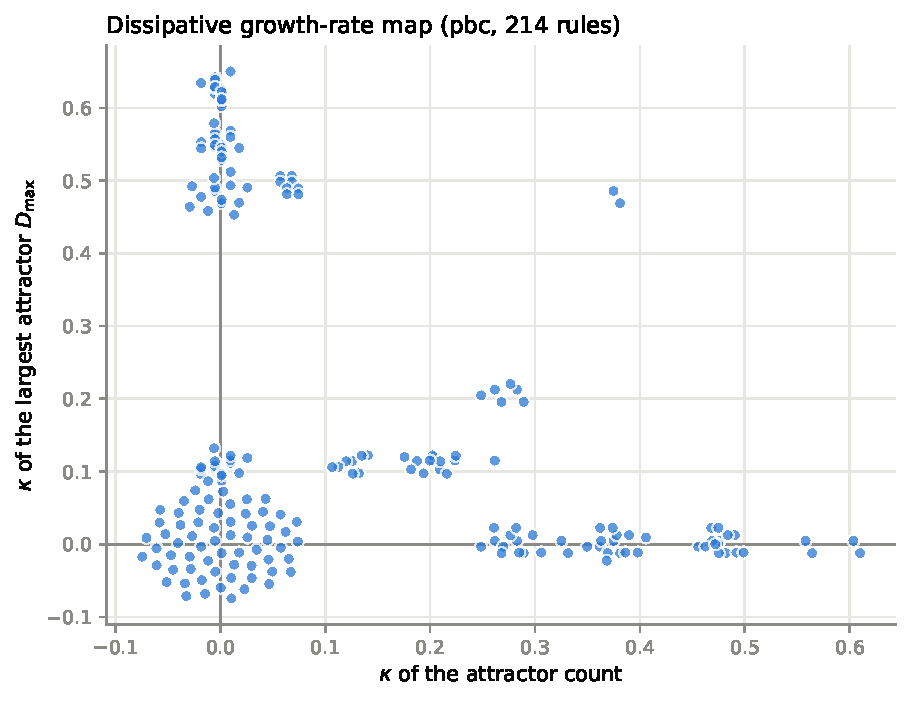
\includegraphics[width=0.78\linewidth]{../../figures/fig_diss_growth_scatter_pbc.pdf}
\caption{Dissipative growth-rate map (pbc): exponential rate of the attractor
count against that of the largest attractor, one point per rule. Coincident
points are spread over a small disc so that they can be counted.}
\label{fig:scatter}\end{figure}

\begin{figure}[h]\centering
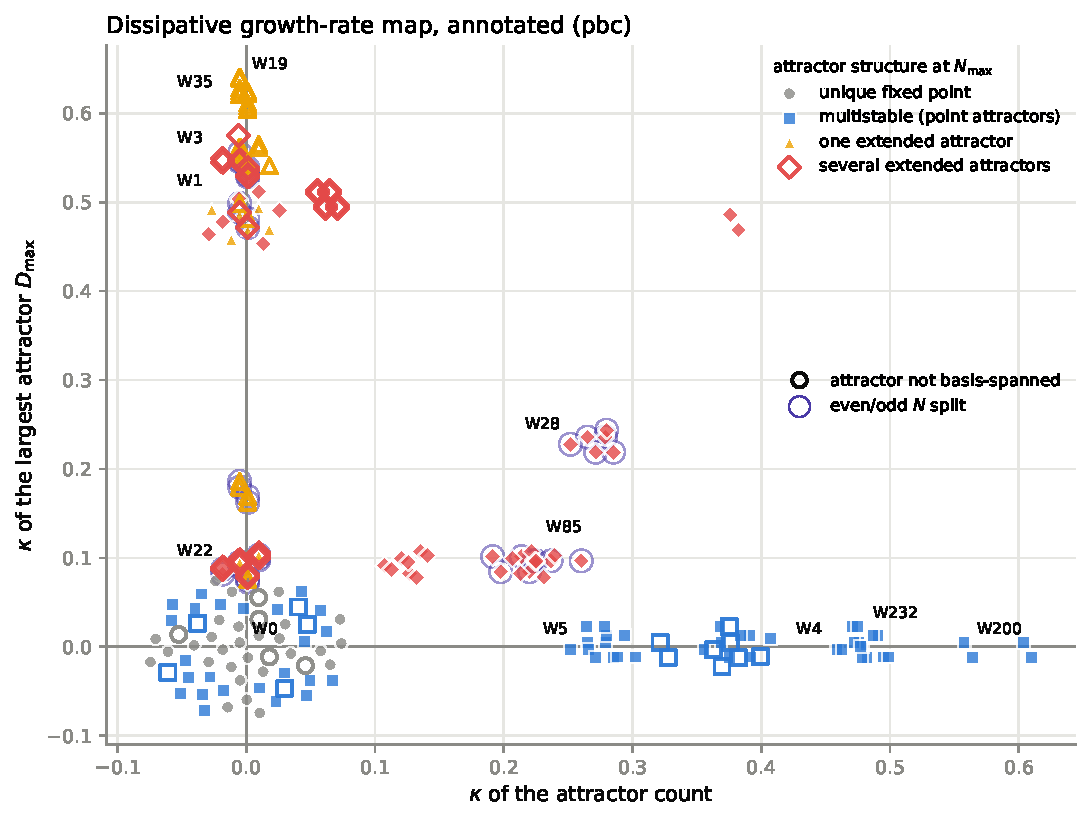
\includegraphics[width=0.95\linewidth]{../../figures/fig_diss_growth_scatter_annot_pbc.pdf}
\caption{The same map, annotated. Hue/marker: graph-level attractor structure at
$N_{\max}$. Hollow ring: the channel attractor is not spanned by basis states, so
no state-space graph can name it. Purple halo: even- and odd-$N$ subsequences
obey different growth laws.}
\label{fig:scatterannot}\end{figure}

\begin{figure}[h]\centering
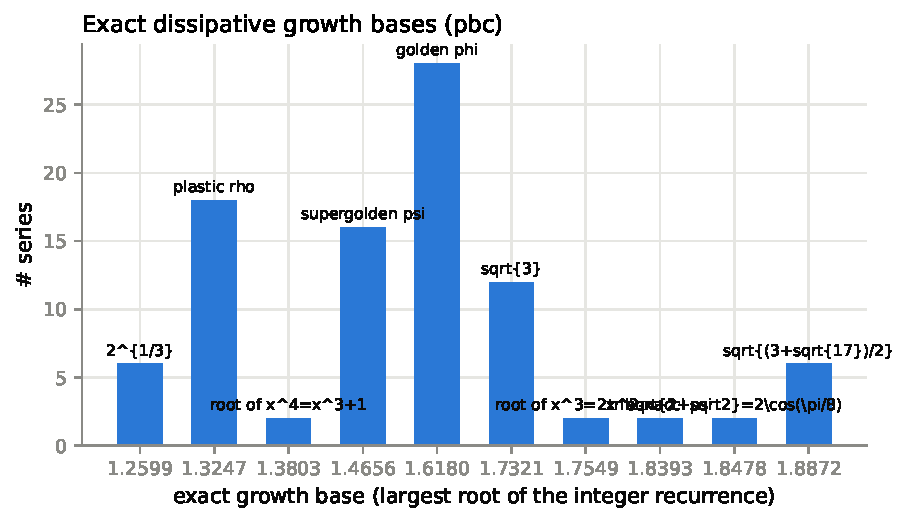
\includegraphics[width=0.78\linewidth]{../../figures/fig_diss_bases_pbc.pdf}
\caption{Exact growth bases (pbc): the largest root of each verified integer
recurrence. The bases are not spread over an interval --- they pile up on a few
algebraic constants.}
\label{fig:bases}\end{figure}

\section{Transient relaxation}
Figure~\ref{fig:depth} shows the transient depth (an exact integer proxy for the
relaxation time) growing with $N$ for representative multistable rules.
\begin{figure}[h]\centering
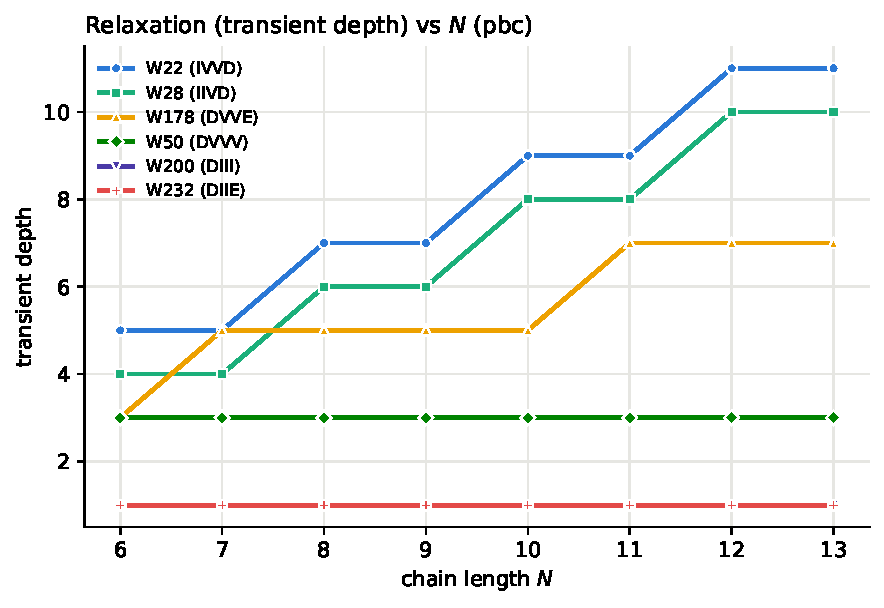
\includegraphics[width=0.7\linewidth]{../../figures/fig_transient_depth_pbc.pdf}
\caption{Transient depth vs.\ $N$ (pbc) for selected dissipative rules.}
\label{fig:depth}\end{figure}

\section{Status and next steps}
The graph-level dissipative classification, the Tier-1b per-class attractor
types, the coherent-attractor census and the Tier-1c growth laws are complete and
checkpointed. The open targets are: (i) whether the wall-Hadamard core's coherent
attractor is a decoherence-free subsystem with a Tier-2 symmetry operator behind
it; (ii) why the coherent count is non-monotonic in $N$ ($84\to60\to72$), which
looks like a parity effect of the same kind as \S\ref{sec:scaling} but is not yet
proved; and (iii) pushing the census beyond $N=8$, currently limited by the
$2^N$ dense $\rho$.

All numbers derive from \rt{results/*.jsonl} (engine\_version \texttt{1a.1}),
\rt{analytics/coherent\_attractor\_census.json}, and
\rt{figures/dissipative\_summary.csv}; regenerated by
\rt{python -m qca\_fragmentation.quantum.dissipative\_report},
\rt{python -m qca\_fragmentation.quantum.attractor\_structure},
\rt{python -m qca\_fragmentation.scaling.dissipative} and
\rt{python -m qca\_fragmentation.scaling.diss\_figure}.

\begin{thebibliography}{9}
\bibitem{mow} O.~Martin, A.~M.~Odlyzko, S.~Wolfram,
\emph{Algebraic properties of cellular automata},
Comm.\ Math.\ Phys.\ \textbf{93} (1984) 219--258.
\bibitem{lindmarcus} D.~Lind, B.~Marcus,
\emph{An Introduction to Symbolic Dynamics and Coding},
Cambridge University Press, 1995 (subshifts of finite type; Perron eigenvalue
$=e^{\text{topological entropy}}$).
\bibitem{prodinger} H.~Prodinger, R.~F.~Tichy,
\emph{Fibonacci numbers of graphs},
Fibonacci Quart.\ \textbf{20} (1982) 16--21 (independent sets of $P_n$/$C_n$
$=$ Fibonacci/Lucas).
\bibitem{transfermatrix} \emph{Counting short trajectories in elementary
cellular automata using the transfer matrix method}, arXiv:2508.09768 (2025).
\bibitem{fibcycles} \emph{Fibonacci cycles and fixed points}, arXiv:2310.04439
(2023).
\bibitem{oeis} OEIS Foundation, \emph{The On-Line Encyclopedia of Integer
Sequences}, \href{https://oeis.org}{oeis.org}: A000045 (Fibonacci), A000032
(Lucas), A000931 (Padovan), A001608 (Perrin), A000930 (Narayana), A000073
(tribonacci).
\bibitem{wolfram} S.~Wolfram, \emph{Statistical mechanics of cellular automata},
Rev.\ Mod.\ Phys.\ \textbf{55} (1983) 601--644.
\end{thebibliography}

\end{document}
